\documentclass{beamer}
%\documentclass[handout,t]{beamer}

\batchmode
% \usepackage{pgfpages}
% \pgfpagesuselayout{4 on 1}[letterpaper,landscape,border shrink=5mm]

\usepackage{amsmath,amssymb,amsfonts,enumerate,epsfig,bbm,calc,color,ifthen,capt-of}

\usetheme{Berlin}
\usecolortheme{mit}
\usefonttheme[onlymath]{serif}

\title{Task-agnostic Continual Learning with Hybrid Probabilistic Models}
\author[Polina Kirichenko \and Mehrdad Farajtabar]{
  Polina Kirichenko \inst{1} \and Mehrdad Farajtabar \inst{2} \and Dushyant Rao \inst{2} \\
  Balaji Lakshminarayanan \inst{3} \and Nir Levine \inst{2} \and Ang Li \inst{2} \\
  Huiyi Hu \inst{2} \and Andrew Gordon Wilson \inst{1} \and Razvan Pascanu \inst{2}
}

\institute[NYU \and DeepMind \and Google Brain]{
  \inst{1} New York University \and
  \inst{2} DeepMind \and
  \inst{3} Google Brain
}
\date{\today}
% \pgfdeclareimage[height=0.5cm]{mit-logo}{mit-logo.pdf}
% \logo{\pgfuseimage{mit-logo}\hspace*{0.3cm}}

% \AtBeginSection[]
% {
%   \begin{frame}<beamer>
%     \frametitle{Outline}
%     \tableofcontents[currentsection]
%   \end{frame}
% }
\beamerdefaultoverlayspecification{<+->}
% -----------------------------------------------------------------------------
\begin{document}
% -----------------------------------------------------------------------------

\frame{\titlepage}

% \section[Outline]{}
% \begin{frame}{Outline}
%   \tableofcontents
% \end{frame}

% -----------------------------------------------------------------------------
\section{Introduction}
% \subsection{Smoot's Ear: The Measure of Humanity}
\begin{frame}{Related Work}
  \textbf{Continual Learning}:
  \begin{itemize}
    \item <1-> Replay-based methods: Store a memory of the examples or knowledge learned so far.
    \item <1-> Regularization-based methods: Constrain the parameter updates while learning new tasks to preserve previous knowledge.
    \begin{itemize}
      \item <1-> EWC, function-space regularization, feature regularization, OGD, AGEM, GPM, \dots
    \end{itemize}
    \item <1-> Modularity-based methods: Allocate different subsets of the parameters to each task.
  \end{itemize}
  % \begin{block}{Title of}
  %   hi
  % \end{block}
\end{frame}

\begin{frame}{Related Work}
  \textbf{Task-Agnostic CL}: The task index is not provided during training and testing.
  \begin{itemize}
    \item <1-> Use the online variational Bayes framework to avoid the need or explicit task identities.
    \item <1-> Detect task changes as peaks in the loss values following a plateau.
    \item <1-> Infer the latent tasks within a Dirichlet process mixture model.
    \item <1-> embed the information associated with different domains into several clusters.
    \item <1-> CURL, CN-DPMM, \dots
  \end{itemize}
\end{frame}

% \begin{frame}{Related Work}
%   \textbf{OOD}:

%   \textbf{Hybrid Models}:
% \end{frame}

\begin{frame}{Related Work}
  \textbf{Normalizing Flows}: a flexible deep generative model with tractable likelihood 
  based on invertible neural networks. Flows model the data distribution $p_X$ as
  \[
    \hat{p}_X = f_\theta^{-1}(\hat{p}_Z),
  \]
  where $\hat{p}_Z$ is a fixed density in the latent space and 
  $f_\theta : \mathcal{X} \rightarrow \mathcal{Z}$ is an invertible neural network.
  $\mathcal{X}$ and $\mathcal{Z}$ have the same dimension. Thus,
  \[
    \hat{p}_X(x) = \hat{p}_Z(f_\theta(x)) \cdot \left| \frac{\partial f_\theta}{\partial x} \right|.
  \]
  The architecture of the flow networks is designed to ensure cheap computation of $f^{-1}$ and $\left| \frac{\partial f_\theta}{\partial x} \right|$,
  such as \emph{NICE}, \emph{RealNVP} and \emph{GLOW}.
\end{frame}

\begin{frame}{The Contributions}
  \begin{itemize}
    \item <1-> Hybrid Continual Learning (HCL) - a normalizing flow-based approach.
    \item Generative replay and a novel functional regularization are employed to alleviate forgetting. The functional regularization is shown to be better than generative replay.
    \item <1-> HCL achieves strong performance on \emph{split MNIST}, \emph{split CIFAR}, \emph{SVHN-MNIST} and \emph{MNIST-SVHN} datasets.
    \item <1-> HCL can detect task boundaries and identify new as well as recurring tasks.
  \end{itemize}
\end{frame}

% -----------------------------------------------------------------------------
\section{Background and Notation}
\begin{frame}{Continual Learning (CL)}
  \begin{itemize}
    \item <1-> A CL model $g_\theta : \mathcal{X} \rightarrow \mathcal{Y}$.
    \item <1-> A sequence of $\tau$ supervised tasks: $T_{t_1}, \ T_{t_2}, \dots, T_{t_\tau}$. $\tau$ is not known in advance.
    \item <1-> Each task $T_i = \{ (x_j^i, y_j^i) \}_{j = 1}^{N_i}$, where $x_j^i \in \mathcal{X}^i$ and $y_j^i \in \mathcal{Y}^i = \{ 1, \dots, K \}$.
    \item <1-> The corresponding data distribution of task $T_i$ is $p_i(x, y)$.
    \item <1-> \textbf{Constraint}: While training on a task $T_i$ the model cannot access to the data from previous $T_1, \dots, T_{i-1}$ or future tasks $T_{i+1}, \dots, T_{\tau}$.
    \item <1-> \textbf{Objective}: Minimize $\sum_{i = 1}^M \mathbb{E}_{x, y \sim p_i(\cdot, \cdot)}l(g_\theta(x), y)$ for some risk function $l(\cdot, \cdot)$ and generalize well on all tasks after training.
  \end{itemize} 
\end{frame}

\begin{frame}{Task-Agnostic CL}
  In this work, the \emph{task-agnostic} setting is considered, where the task index is not provided and the model has to infer it from data.
  Besides, some of the tasks can be recurring.
\end{frame}

% -----------------------------------------------------------------------------
\section{HCL}
\begin{frame}{An illustration of the HCL Framework}
  \begin{figure}
    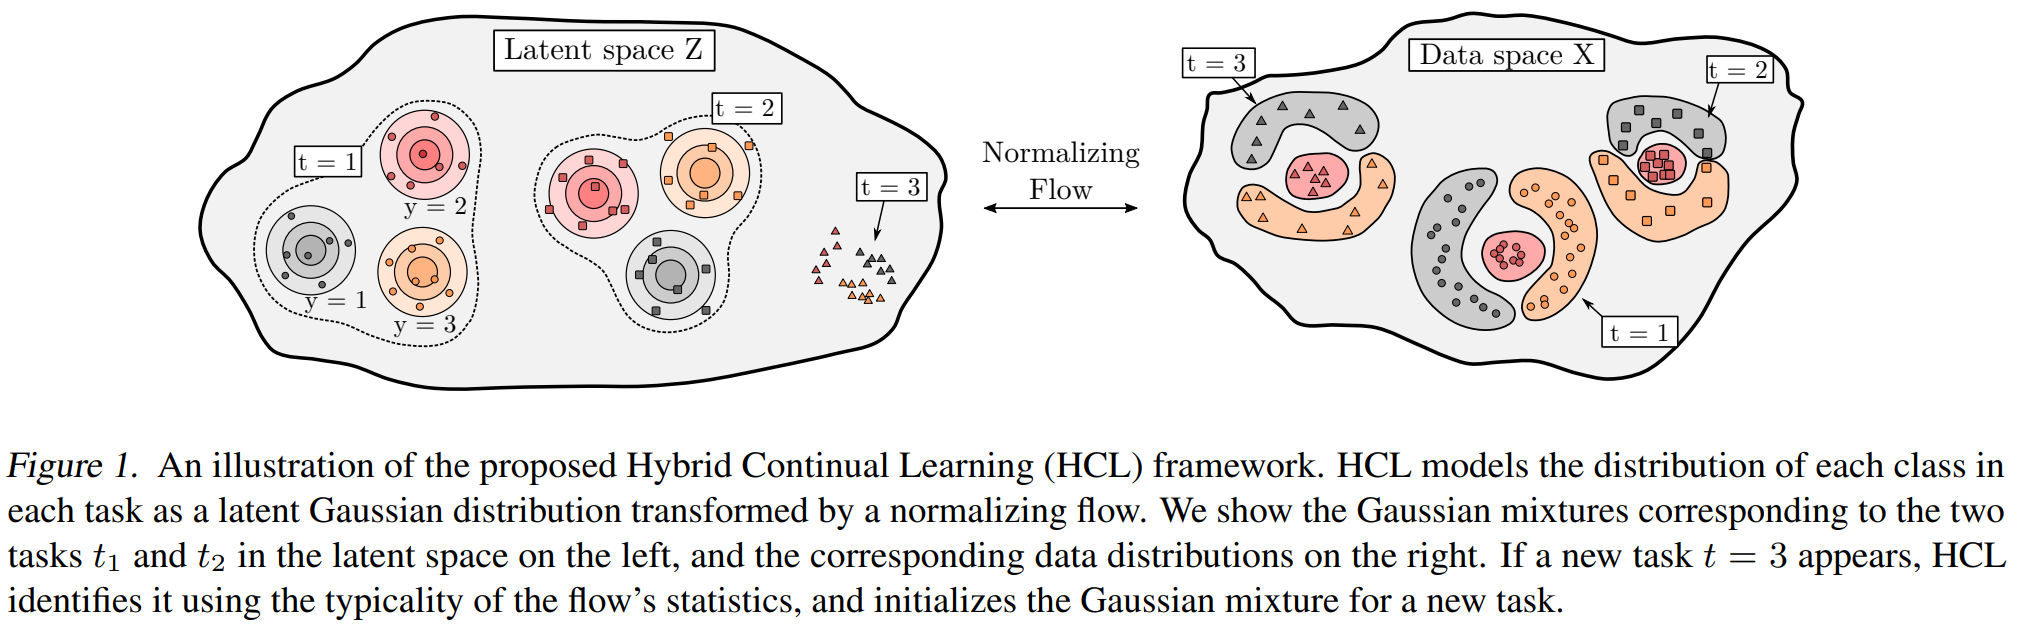
\includegraphics[width=1\textwidth]{./figures/Model_illustration}
  \end{figure}
\end{frame}

\begin{frame}{Modeling the Data Distribution}
  \begin{itemize}
    \item <1-> $p_t(x, y)$: the joint distribution of the data $x$ and the class label $y$ conditioned on a task $t$.
    \[
      p_t(x, y) \approx \hat{p}(x, y | t) = \hat{p}_X(x | y, t) \hat{p}(y | t)
    \]
    \item <1-> $\hat{p}_X(x | y, t)$ is modeled by a normalizing flow $f_\theta$ with a base distribution $\hat{p}_Z = \mathcal{N}(\mu_{y, t}, I)$.
    \[
      \hat{p}_X(x | y, t) = f_\theta^{-1}\left( \mathcal{N}(\mu_{y, t}, I) \right)
    \]
    \item <1-> $\mu_{y, t}$ is the mean of the latent distribution corresponding to the class $y$ and task $t$.
    \item <1-> $\hat{p}(y | t)$ is assumed to be a uniform distribution over the classes for each task: $\hat{p}(y | t) = 1/K$.
  \end{itemize}
\end{frame}

\begin{frame}{Task Identification}
  Three statistics on data batches $B$.
  \begin{itemize}
    \item <1-> log-likelihood
    \[
      S_1(B, t) = \sum_{(x_j, y_j) \in B} \hat{p}_X(x_j | y_j, t)
    \]
    \item <1-> log-likelihood of the latent variable 
    \[
      S_2(B, t) = \sum_{(x_j, y_j) \in B} \hat{p}_Z(f_\theta(x_j) | y_j, t)
    \]
    \item <1-> log-determinant of the Jacobian
    \[
      S_3(B, t) = S_1(B, t) - S_2(B, t)
    \]
  \end{itemize}
\end{frame}

\begin{frame}{Task Identification}
  \begin{itemize}
    \item <1-> For each task $t$, keep track of the mean $\mu_S^t$ and standard deviation $\sigma_S^t$ for the statistics over a window of the last $l$ batches of data.
    \item <1-> If all the statistics $|S(B, t^\prime) - \mu_S^{t^\prime}| < \lambda \sigma_S^{t^\prime}$ for one of the previous tasks, identify a switch to the task $t^\prime$.
    \item <1-> Otherwise, switch to a new task and add new Gaussians for this task in the latent space.
  \end{itemize}
\end{frame} 

\begin{frame}{Generative Replay (HCL-GR)}
  \begin{itemize}
    \item <1-> Store a single snapshot of the HCL model $\hat{p}_X^{(k)}(x | y, t)$ with weights $\theta^{(k)}$.
    \item <1-> Generate and replay data from old tasks using the snapshot: $x_{GR} \sim \hat{p}_X^{(k)}(x | y, t)$, where $y \sim U\{1, \dots, K\}$ and $t \sim U\{t_1, \dots, t_k\}$.
    \item <1-> Maximize the likelihood $\mathcal{L}_{GR} = \log \hat{p}_X (x_{GR} | y, t)$ under the current model $\hat{p}_X(\cdot)$.
    \item <1-> The resulting loss in generative replay training is $\mathcal{L}_{ll} + \mathcal{L}_{GR}$, where $\mathcal{L}_{ll}$ is the log-likelihood of the data on the current task.
    \item <1-> Update the snapshot with new weights $\theta^{(k+1)}$ after detecting the task change $T_{t_{k+1}} \rightarrow T_{t_{k+2}}$. 
  \end{itemize}
\end{frame}

\begin{frame}{Functional Regularization (HCL-FR)}
  Enforce the flow to map samples from previous tasks to the same latent representations as a snapshot model.

  \begin{itemize}
    \item <1-> Store a single snapshot of the model $\hat{p}_X^{(k)}(\cdot)$ and produce samples $x_{FR} \sim \hat{p}_X^{(k)}(x | y, t)$ for $y \sim U\{1, \dots, K\}$, $t \sim U\{t_1, \dots, t_k\}$.
    \item <1-> $\mathcal{L}_{FR} = \left\| f_\theta(x_{FR}) - f_{\theta^{(k)}}(x_{FR}) \right\|^2$, where $f_\theta$ is the current flow mapping and $f_{\theta^{(k)}}$ is the snapshot model.
    \item <1-> The resulting loss in functional regularization is $\mathcal{L}_{ll} + \alpha \mathcal{L}_{FR}$.
  \end{itemize}
\end{frame}

% -----------------------------------------------------------------------------
\section{Experiments}
\begin{frame}{Compared Methods}
  \begin{itemize}
    \item <1-> Adam: Train the model with Adam optimizer without any extra steps for preventing forgetting.
    \item <1-> Multi-Task Learning (MTL): When training on $T_{t_i}$, it has access to all previous tasks $T_{t_1}, \dots, T_{t_{i-1}}$.
    \item <1-> Experience Replay (ER): Reserve a buffer with a fixed size of 1000 samples for each task and randomly select samples to add to that buffer during training on each task.
    \item <1-> CURL: CURL incorporated a generative model (VAE) with an expanding Gaussian mixture in latent space and likelihood-based task-change detection.
  \end{itemize}
\end{frame}

\begin{frame}{Datasets}
  \begin{itemize}
    \item <1-> Split MNIST: Split the dataset into 5 binary classification tasks. The epoch is set to 30 for each task. The \emph{Glow} architecture is used to model the data distribution.
    \item <1-> MNIST-SVHN and SVHN-MNIST: The size of the MNIST images is upscaled to $32 \times 32 \times 3$. The \emph{RealNVP} architecture is used to model the data distribution. The epoch is set to 90 for each task.
    \item <1-> Split CIFAR: Each task corresponds to 2 classes of CIFAR-10 and 10 classes of CIFAR-100 respectively. The image embeddings are used, which are extracted by an EfficientNet model pre-trained on ImageNet. The epoch is set to 15 for each task. The \emph{RealNVP} architecture is used.
  \end{itemize}
\end{frame}

\begin{frame}{Metrics}
  $a_{i, j}$ : The accuracy of the model on task $i$ after training on $j$ tasks.

  \begin{itemize}
    \item <1-> Final accuracy on each task: $a_{i, \tau}$, $i \in \{ 1, \dots, \tau \}$.
    \item <1-> Average final accuracy across tasks: $\frac{1}{\tau} \sum_{i = 1}^\tau a_{i, \tau}$.
    \item <1-> Average forgetting: $\frac{1}{\tau - 1} \sum_{i = 1}^{\tau - 1} (a_{i, i} - a_{i, \tau})$.
    \item <1-> Overall accuracy: the final accuracy on $(K \times \tau)$ - way classification.
  \end{itemize}
\end{frame}

\begin{frame}{Experiment Results}
  \begin{figure}
    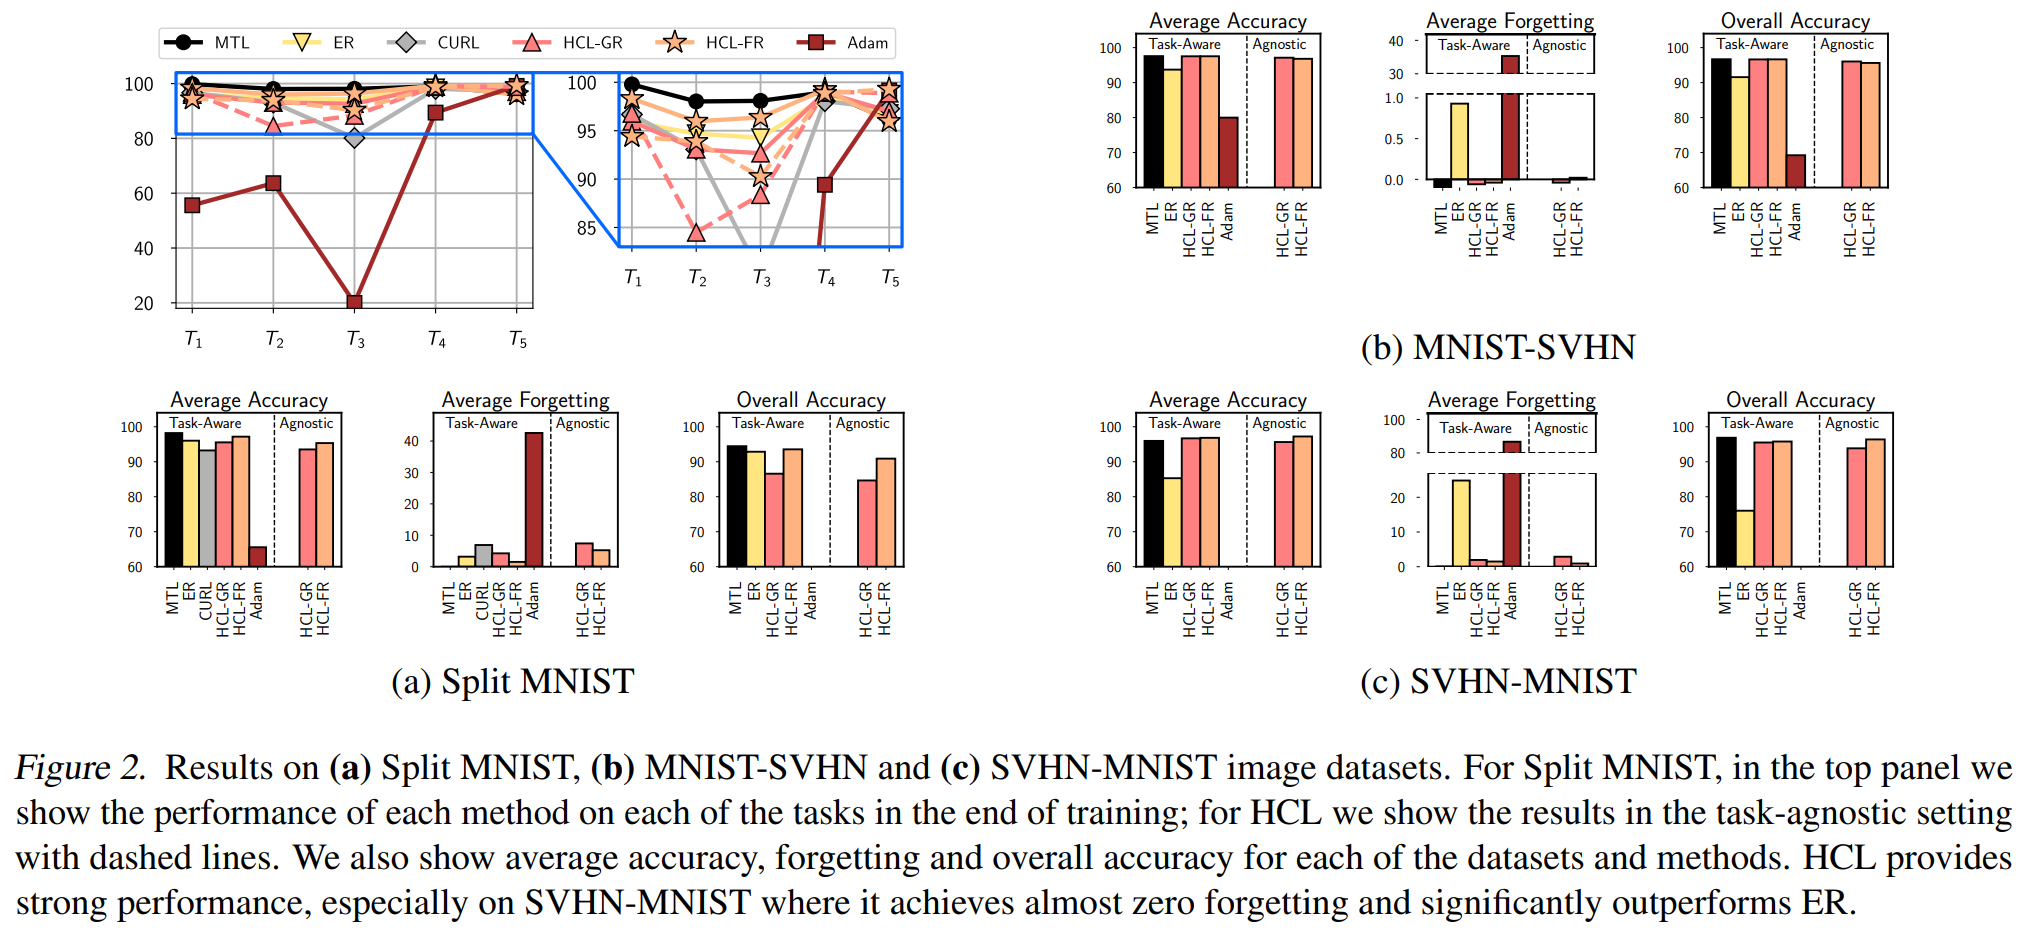
\includegraphics[width=1\textwidth]{./figures/Experiment_result_on_MNIST}
  \end{figure}
\end{frame}

\begin{frame}{Experiment Results}
  \begin{figure}
    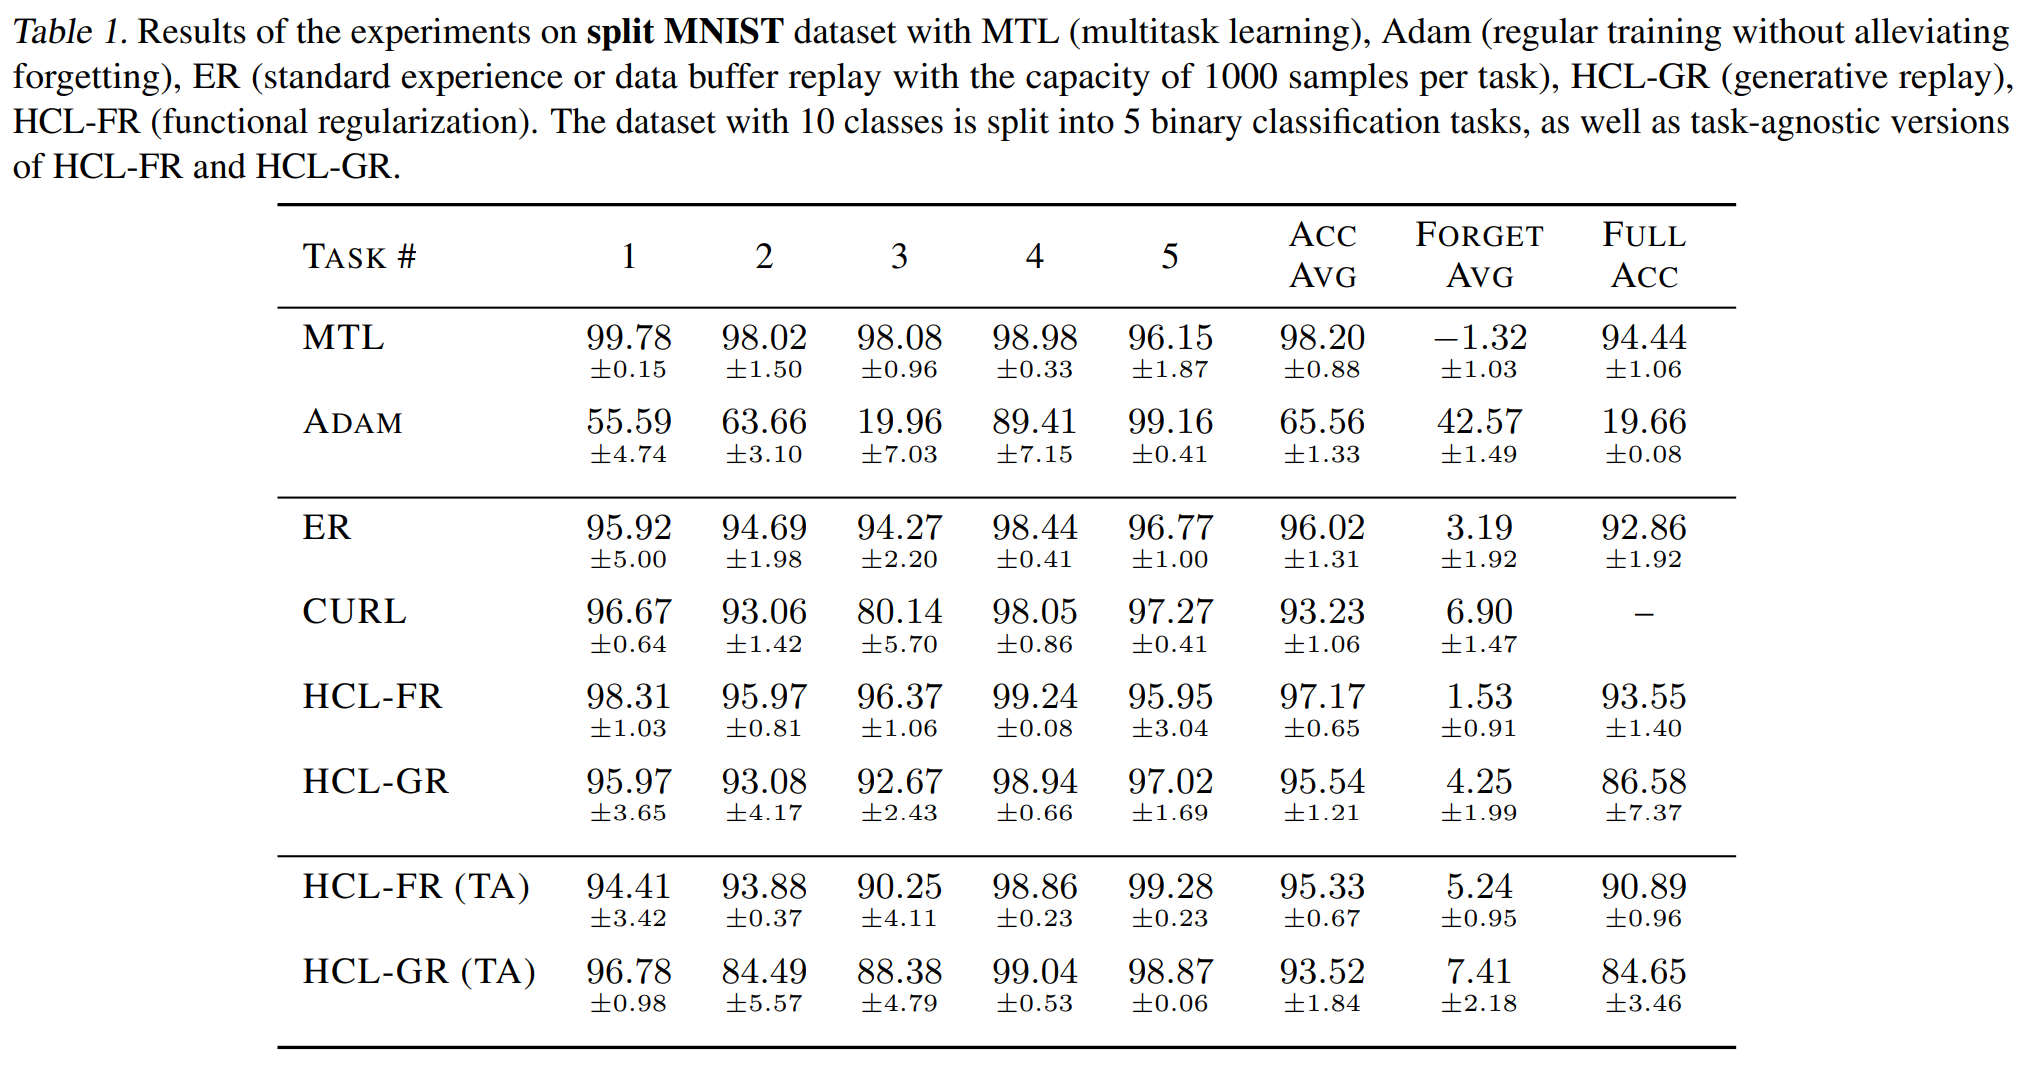
\includegraphics[width=1\textwidth]{./figures/Split_MNIST_Results}
  \end{figure}
\end{frame}

\begin{frame}{Experiment Results}
  \begin{figure}
    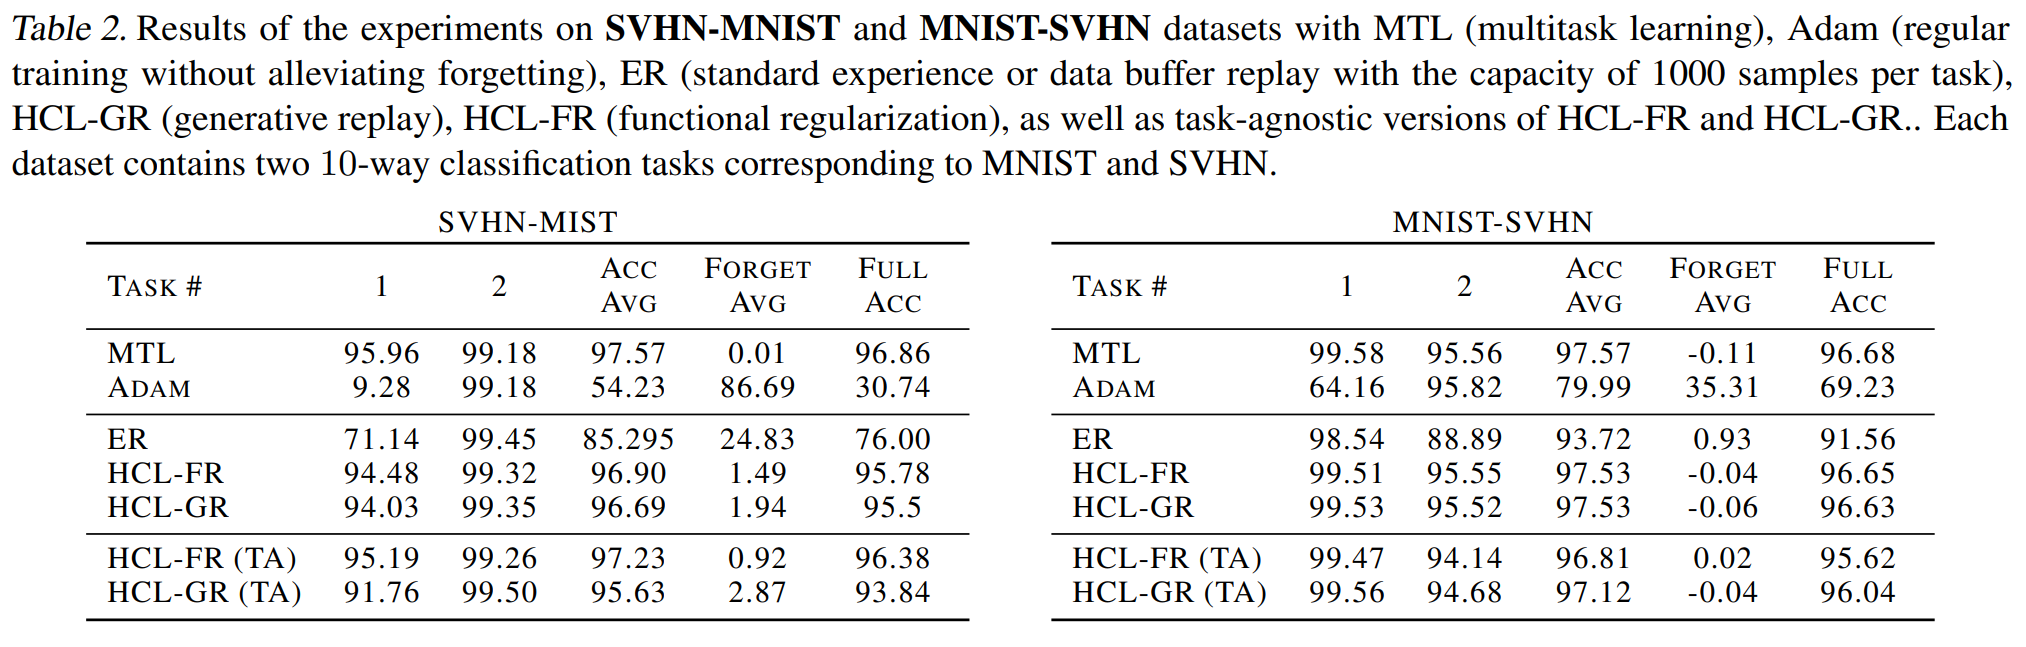
\includegraphics[width=1\textwidth]{./figures/MNIST_SVHN_Results}
  \end{figure}
\end{frame}

\begin{frame}{Experiment Results on Split CIFAR}
  \begin{figure}
    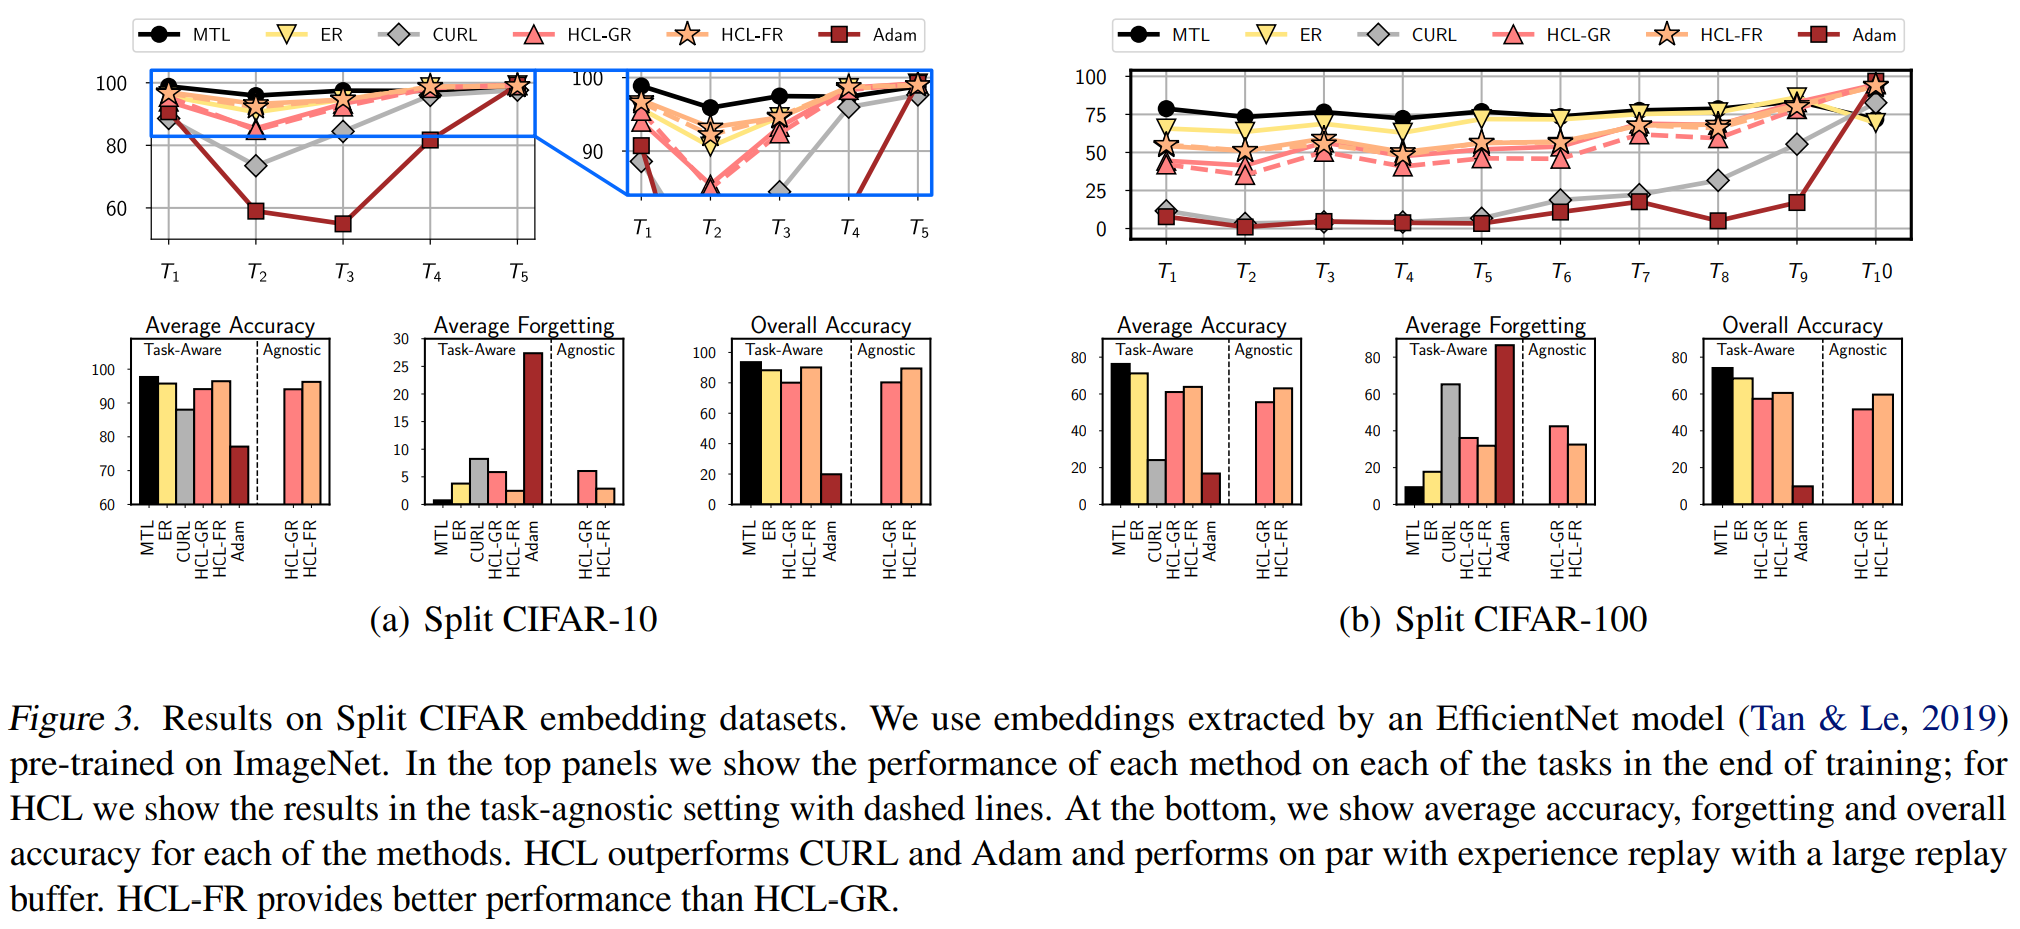
\includegraphics[width=1\textwidth]{./figures/Experiment_result_on_CIFAR}
  \end{figure}
\end{frame}

\begin{frame}{Experiment Results on Split CIFAR-10}
  \begin{figure}
    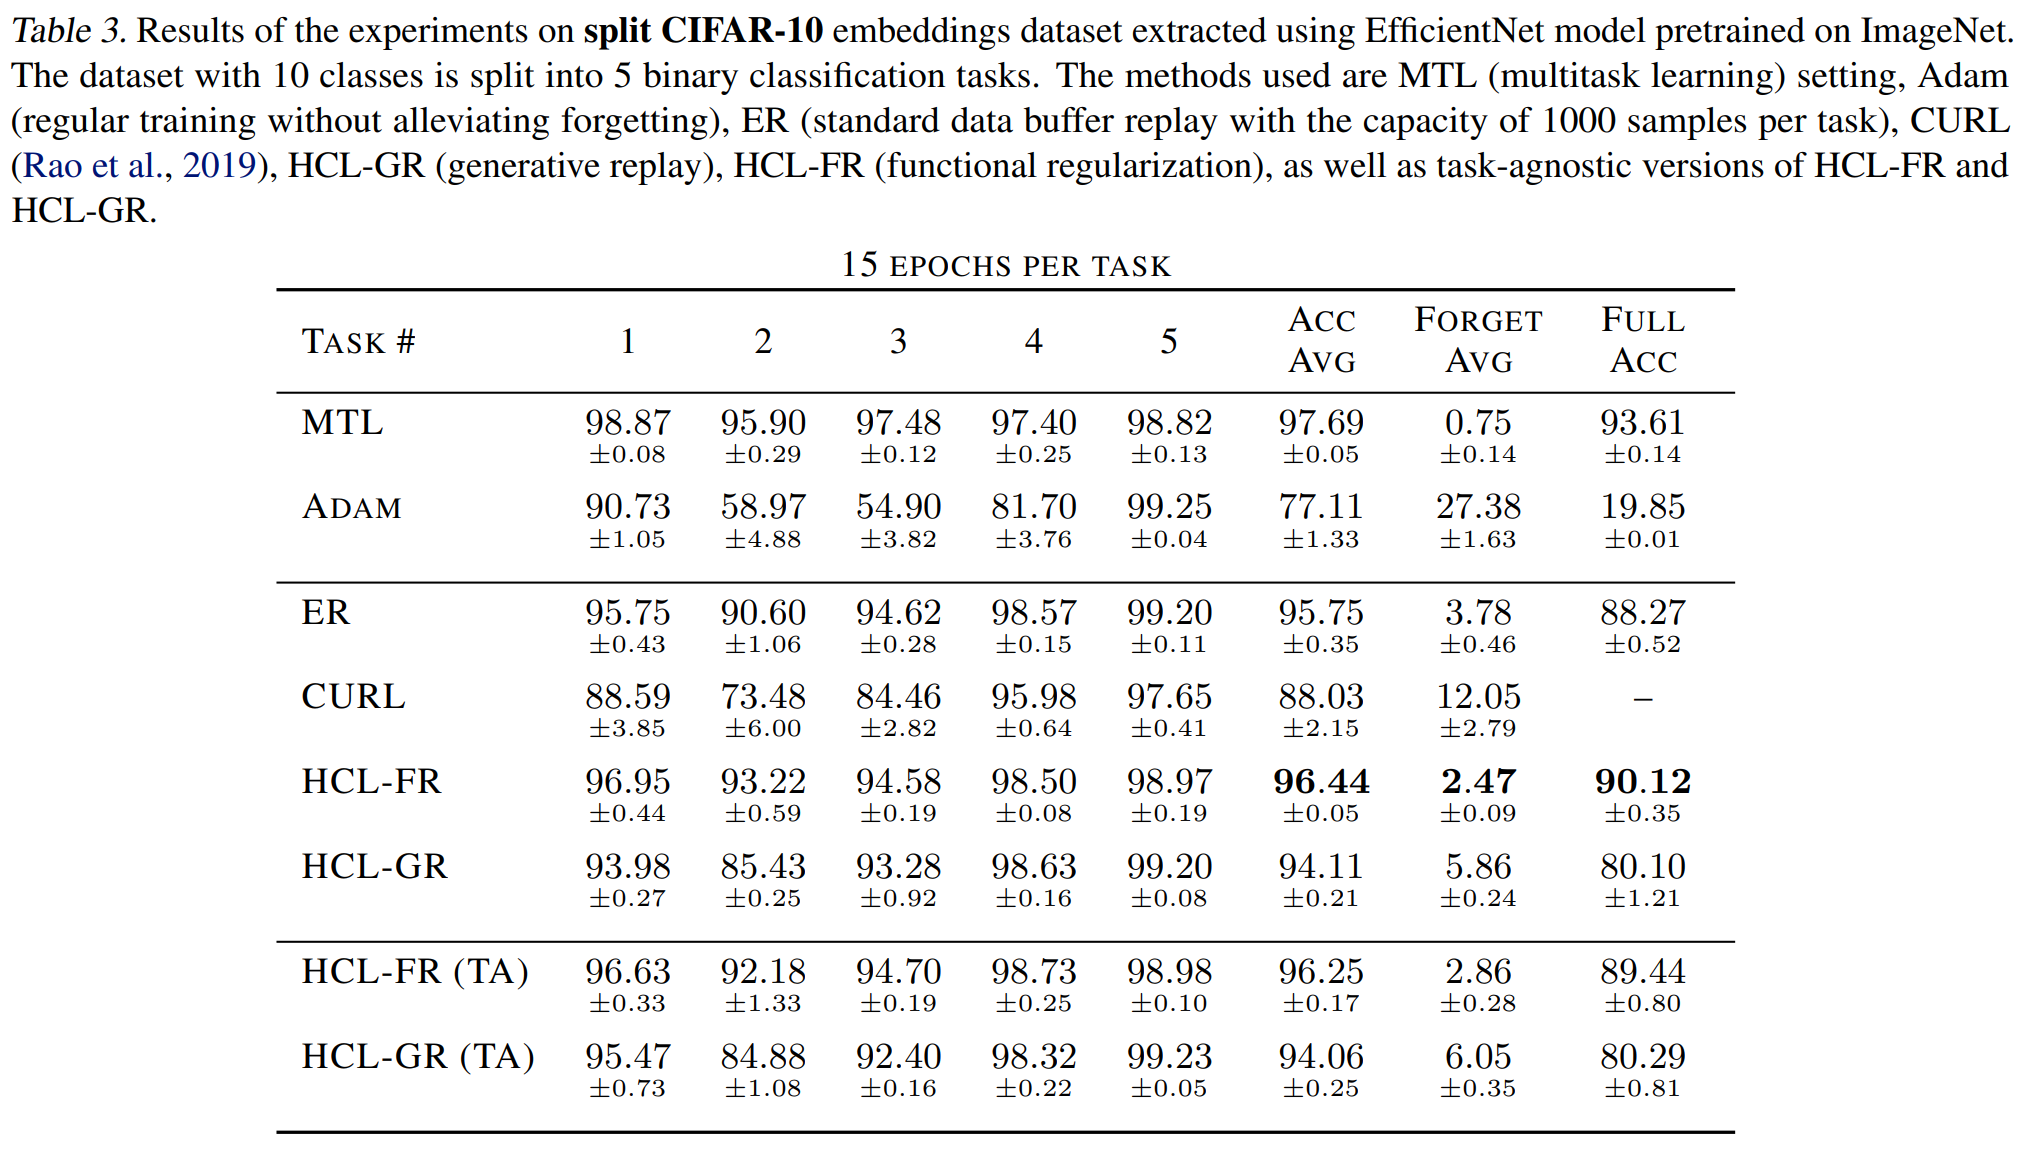
\includegraphics[width=1\textwidth]{./figures/Split_CIFAR10_Results}
  \end{figure}
\end{frame}

\begin{frame}{Experiment Results on Split CIFAR-10}
  \begin{figure}
    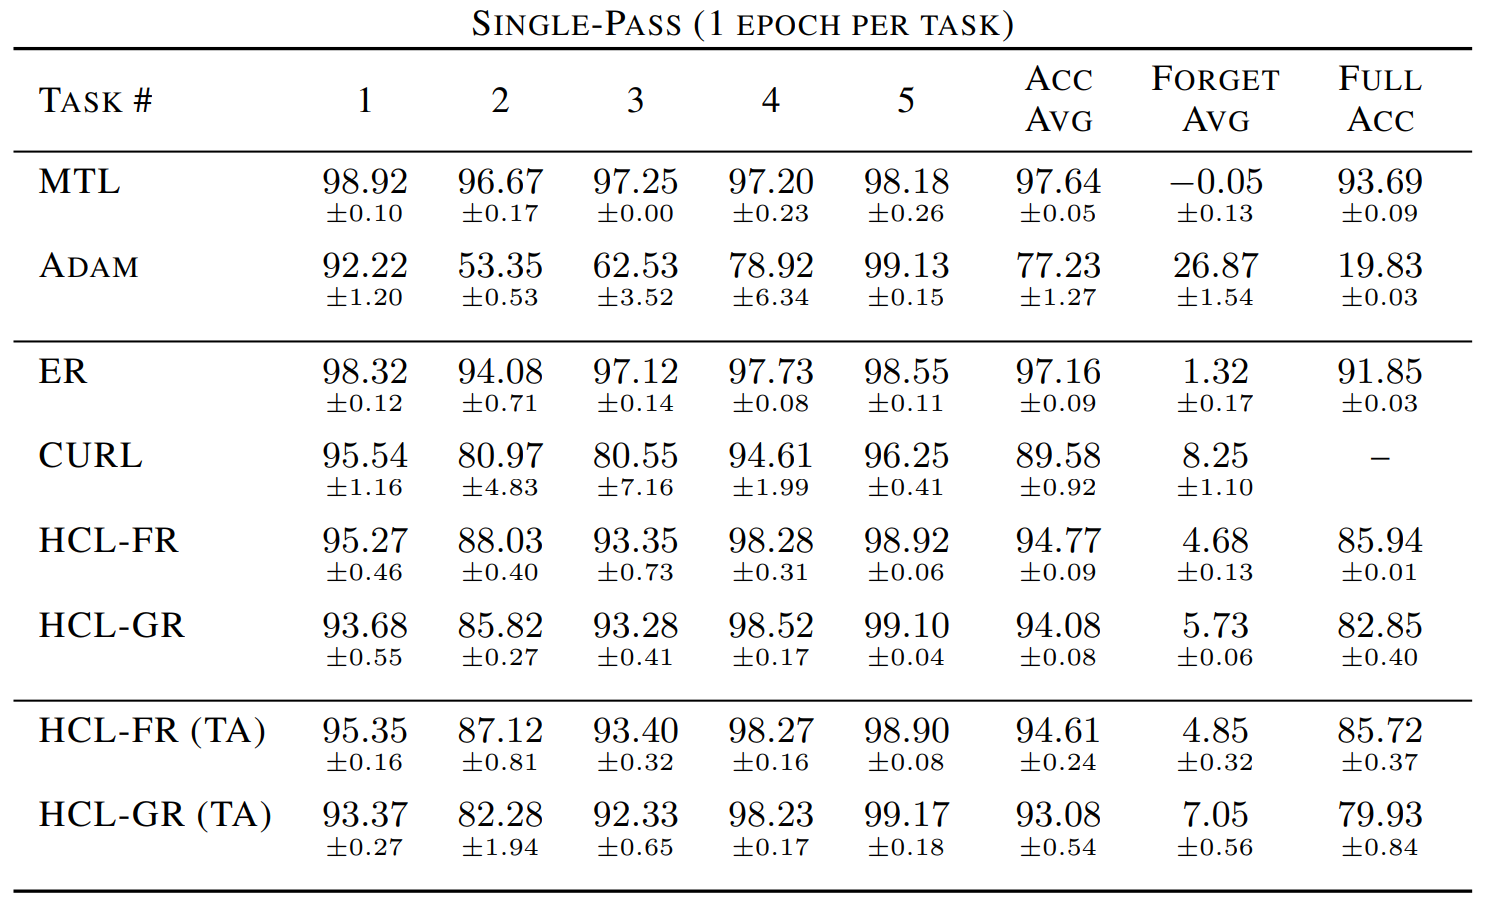
\includegraphics[width=1\textwidth]{./figures/Split_CIFAR10_Results_}
  \end{figure}
\end{frame}

\begin{frame}{Experiment Results on Split CIFAR-100}
  \begin{figure}
    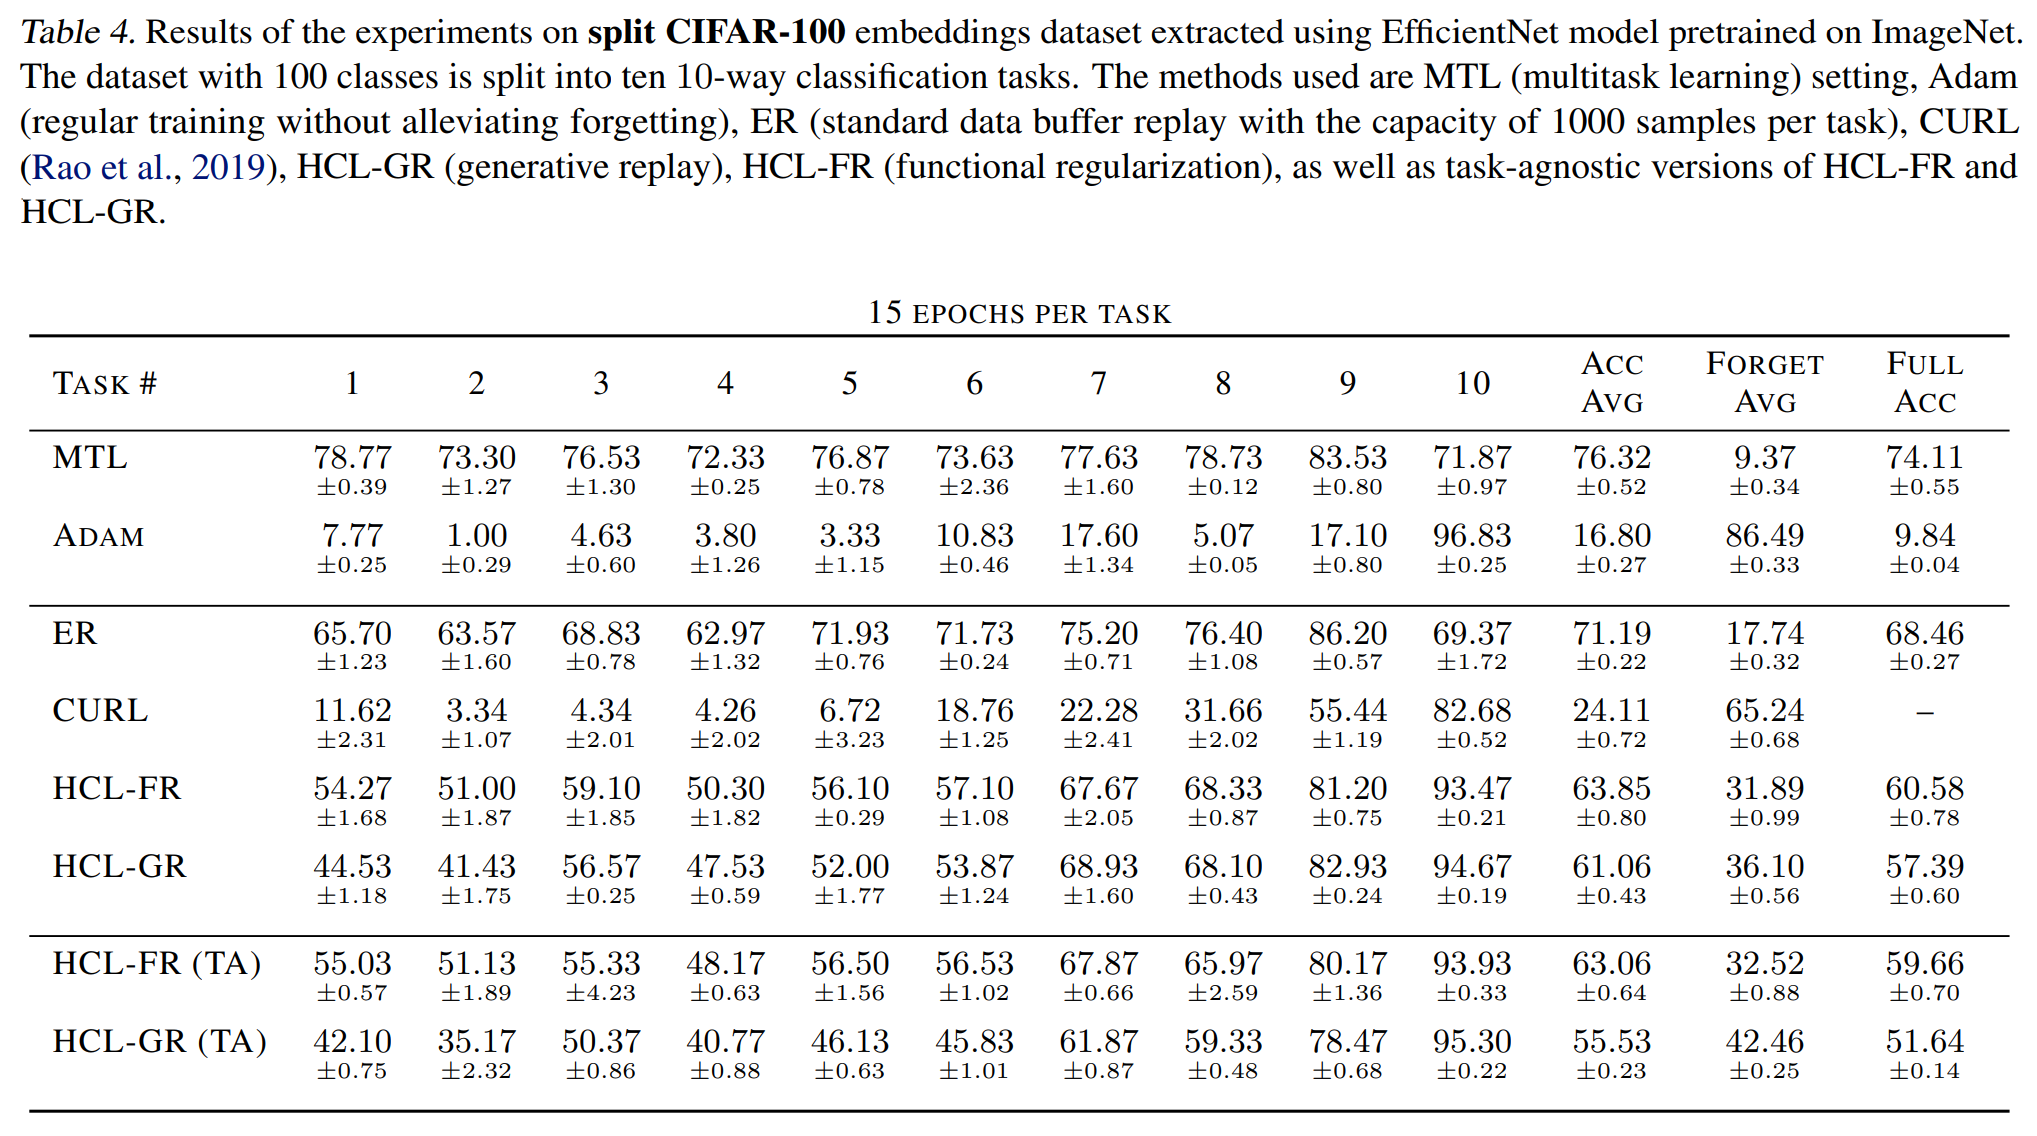
\includegraphics[width=1\textwidth]{./figures/Split_CIFAR100_Results}
  \end{figure}
\end{frame}

\begin{frame}{Experiment Results on Split CIFAR-100}
  \begin{figure}
    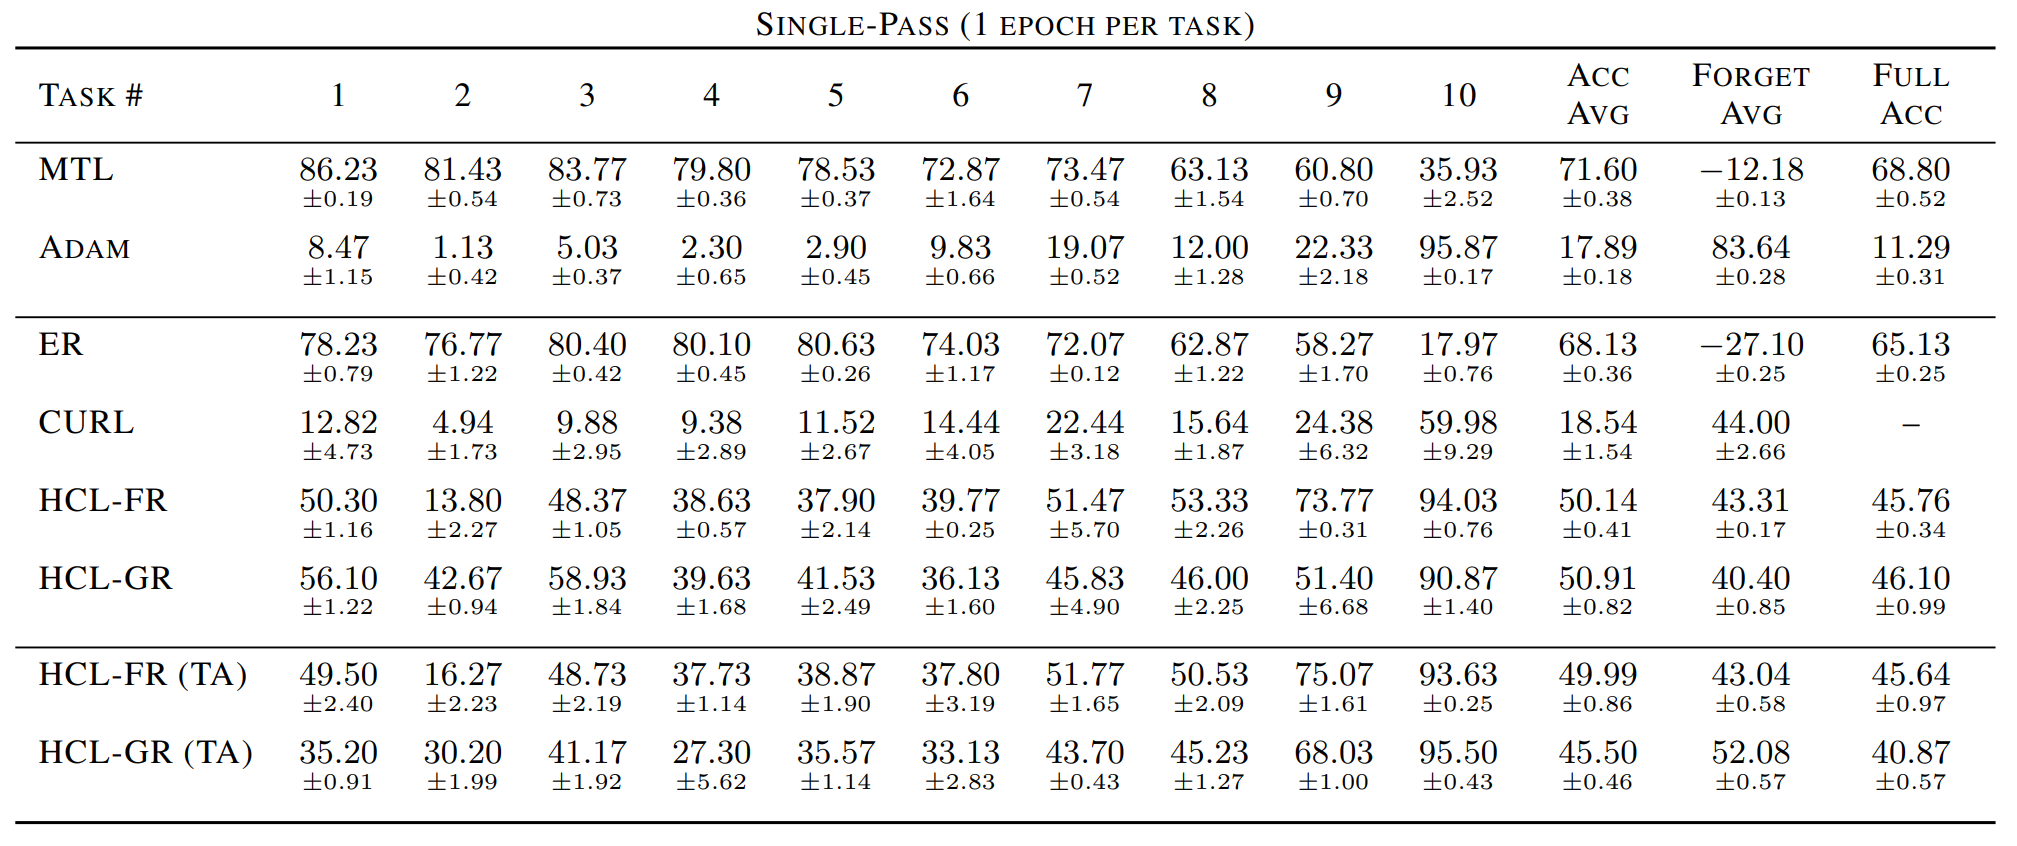
\includegraphics[width=1\textwidth]{./figures/Split_CIFAR100_Results_}
  \end{figure}
\end{frame}

\begin{frame}{Comparison of FR and GR}
  \begin{figure}
    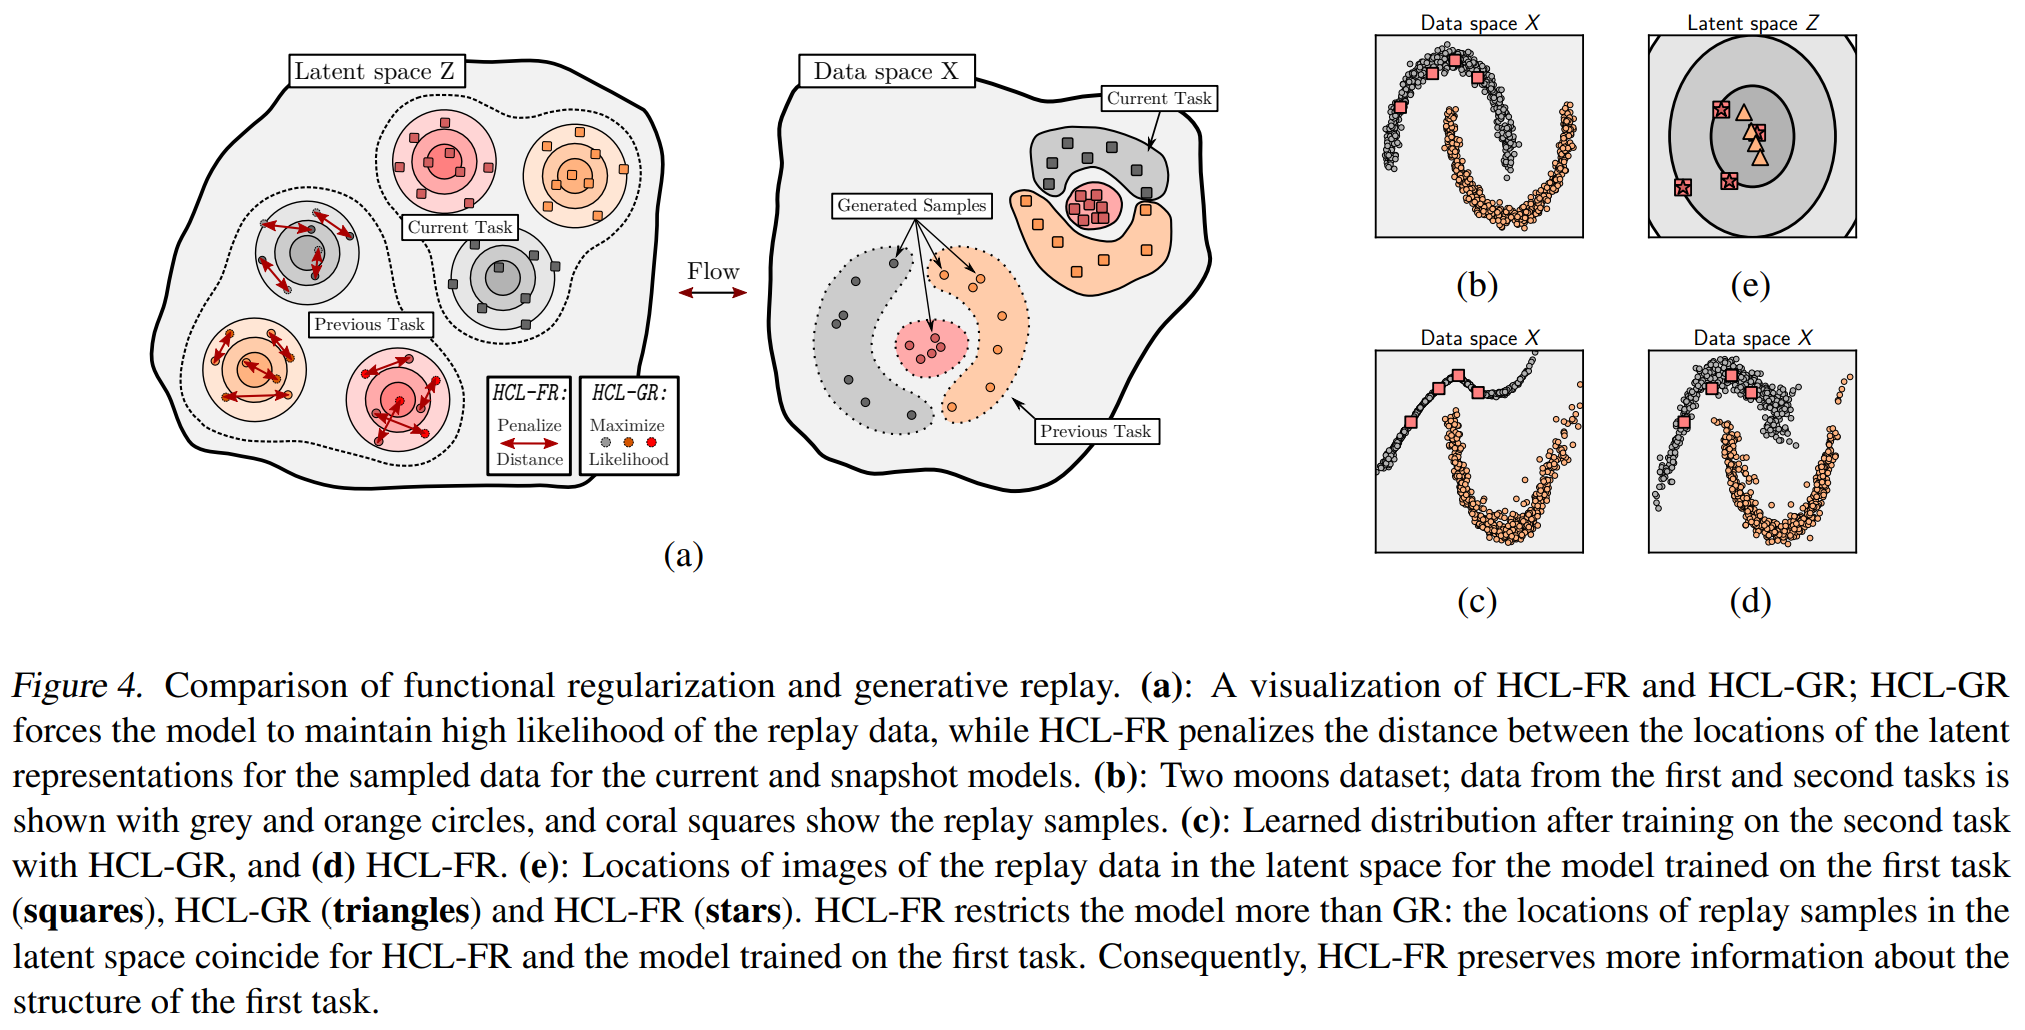
\includegraphics[width=1\textwidth]{./figures/Comparison_FR_GR}
  \end{figure}
\end{frame}

% -----------------------------------------------------------------------------
\section{end}
\begin{frame}
  \centering \large Thanks!
\end{frame}

% -----------------------------------------------------------------------------
\end{document}
